\chapter{Experimentos} \label{cap:experimentos}
%\section{Conclusiones} \label{s:conclusiones}
En este capitulo mostraremos las pruebas realizadas con la herramienta SLAMTESTBED.
Para comprobar los resultados podremos utilizar la ventana que muestra el resultado de las estimaciones una vez han terminado los cálculos. Gracias a la visualización gráfica de los datasets (incluido el dataset estimado) la evaluación de los resultados será más sencilla y fiable, ya que si los puntos 3D del dataset estimado no se aproximan al dataset destino, el desajuste entre los puntos 3d de ambos dataset será perceptible a simple vista.


Acontinuación mostraremos las pruebas realizadas para estimar las transformaciones para convertir el dataset A en el datasetB y viceversa, donde el datasetB se obtiene como resultados de aplicar el módulo transformador sobre el datasetA.
Se han realizado varias pruebas, en cada una de ellas se han activado un subconjunto de parámetros del módulo transformador, es decir que en una prueba se habrá modificado sólo la escala y un traslación , en otras pruebas se habrá realizado cambios en traslación y rotación , etc.

En cada captura de pantalla aparecerá de forma gráfica , el dataset original (en verde), el dataset transformado (en azul), y el dataset estimado (en rojo), junto con otras 3 pantallas que indicarán los valores de los parámetros de las transformaciones realizadas, y otras 2 pantallas con los valores de la estimaciones calculadas (tanto si la estimación ha sido calculada del datasetA al datasetB o del datasetB al datasetA).


\begin{figure}[H]
\begin{center}
\subfigure[]{\label{fig:opciones de View}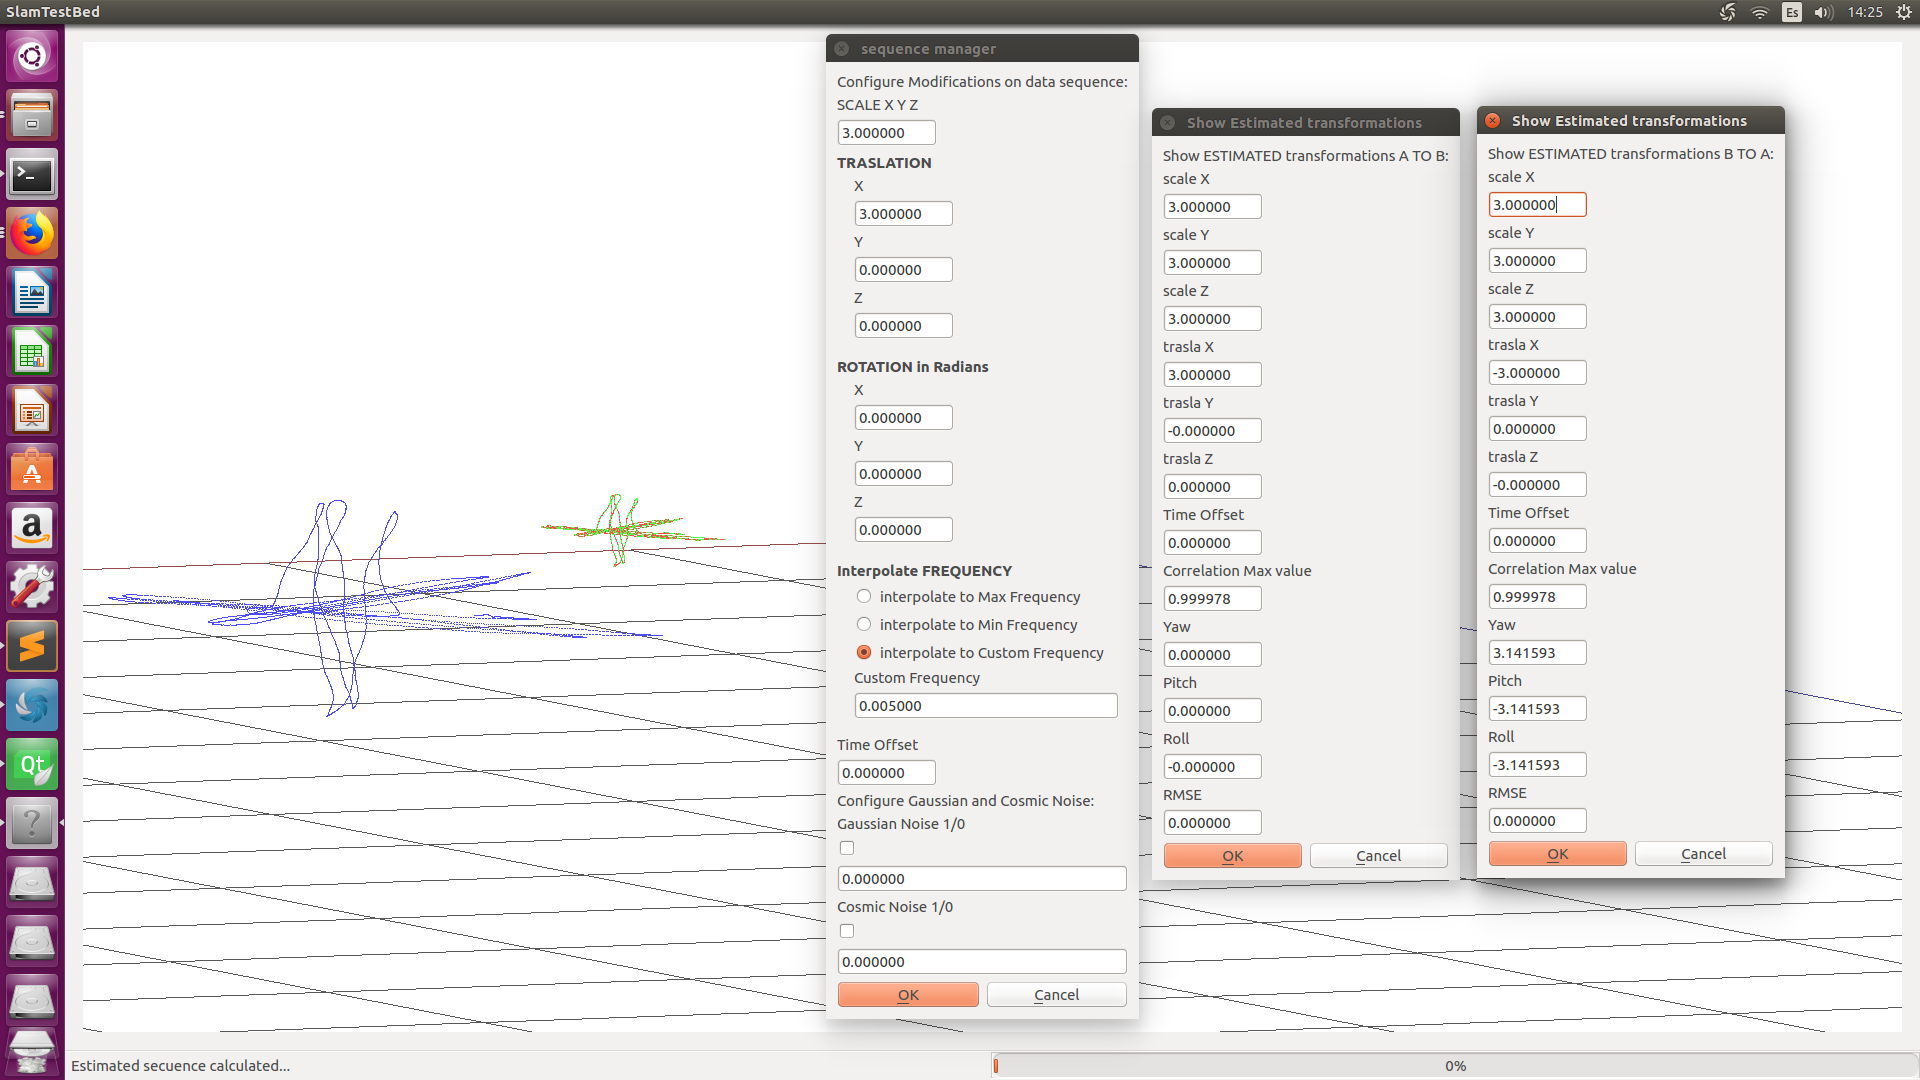
\includegraphics[height=8.0cm,width=12.0cm]{img/cap6/ScaleTraslaFrec.png}}
\hspace{0.5cm}

\end{center}

\caption{Gráfico que muestra los resultados de la estimación de un cambio de escala, traslación y frecuencia.}
\end{figure}


\begin{figure}[H]
\begin{center}
\subfigure[]{\label{fig:opciones de View}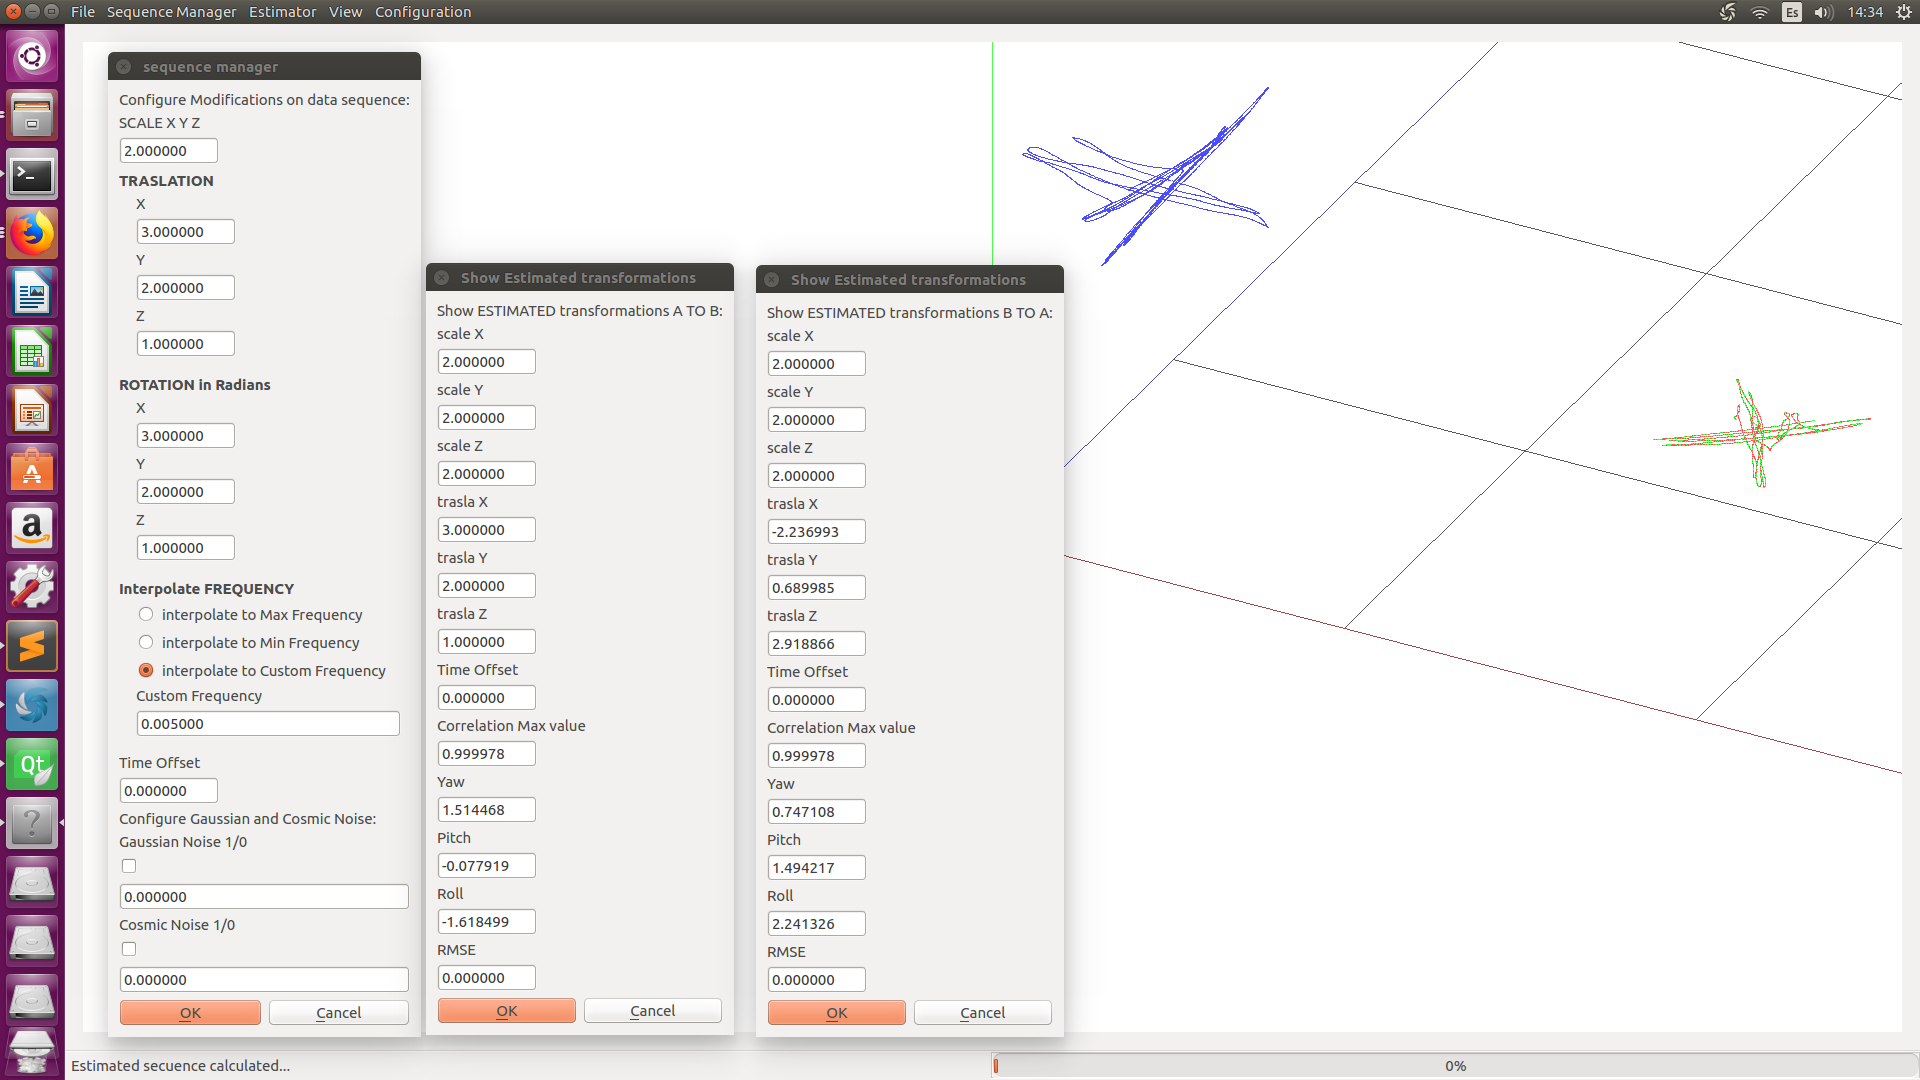
\includegraphics[height=8.0cm,width=12.0cm]{img/cap6/ScaleTraslaRotaFrec.png}}
\hspace{0.5cm}

\end{center}

\caption{Gráfico que muestra los resultados de la estimación de un cambio de escala, traslación,rotación y frecuencia.}
\end{figure}


\begin{figure}[H]
\begin{center}
\subfigure[]{\label{fig:opciones de View}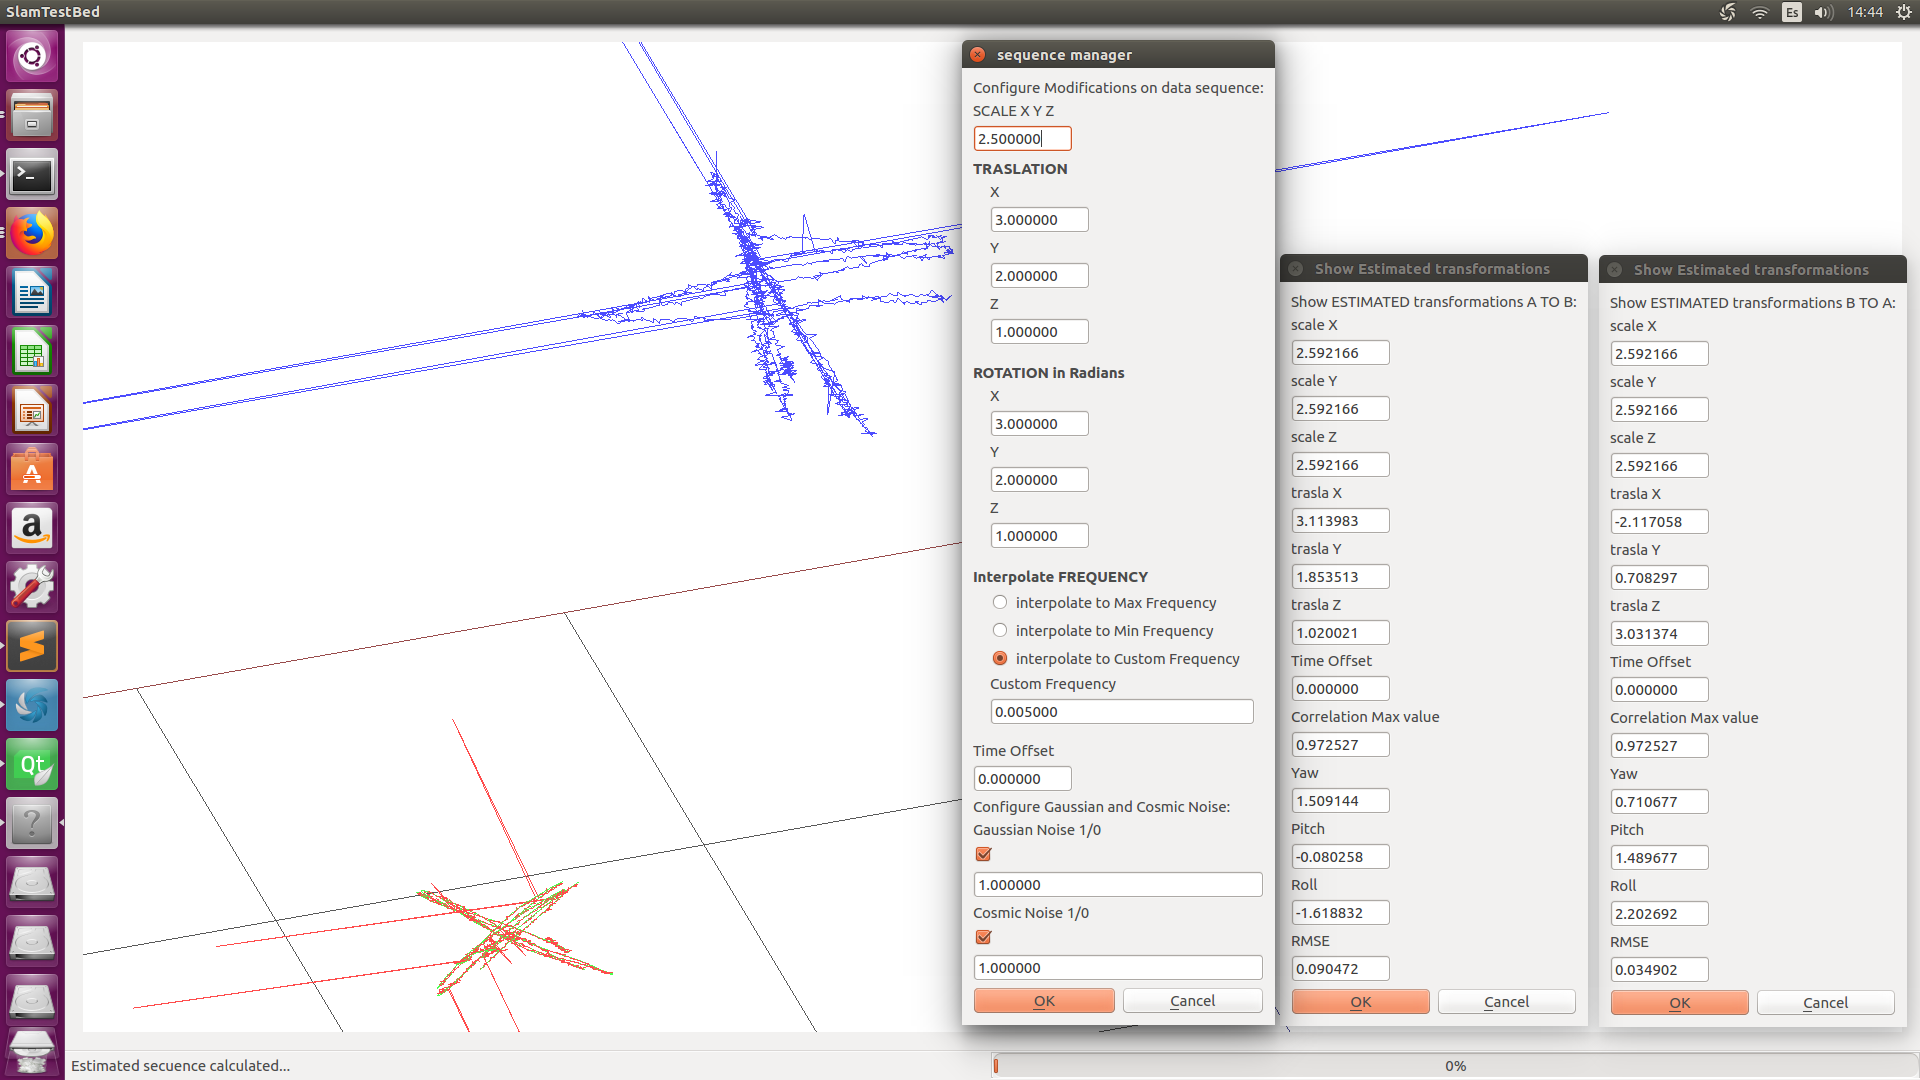
\includegraphics[height=8.0cm,width=12.0cm]{img/cap6/ScaleTraslaRotaFrecGNoiseCNoise.png}}
\hspace{0.5cm}

\end{center}

\caption{Gráfico que muestra los resultados de la estimación de un cambio de escala, traslación, rotación, frecuencia, ruido gaussiano y ruido cósmico.}
\end{figure}



\begin{figure}[H]
\begin{center}
\subfigure[]{\label{fig:opciones de View}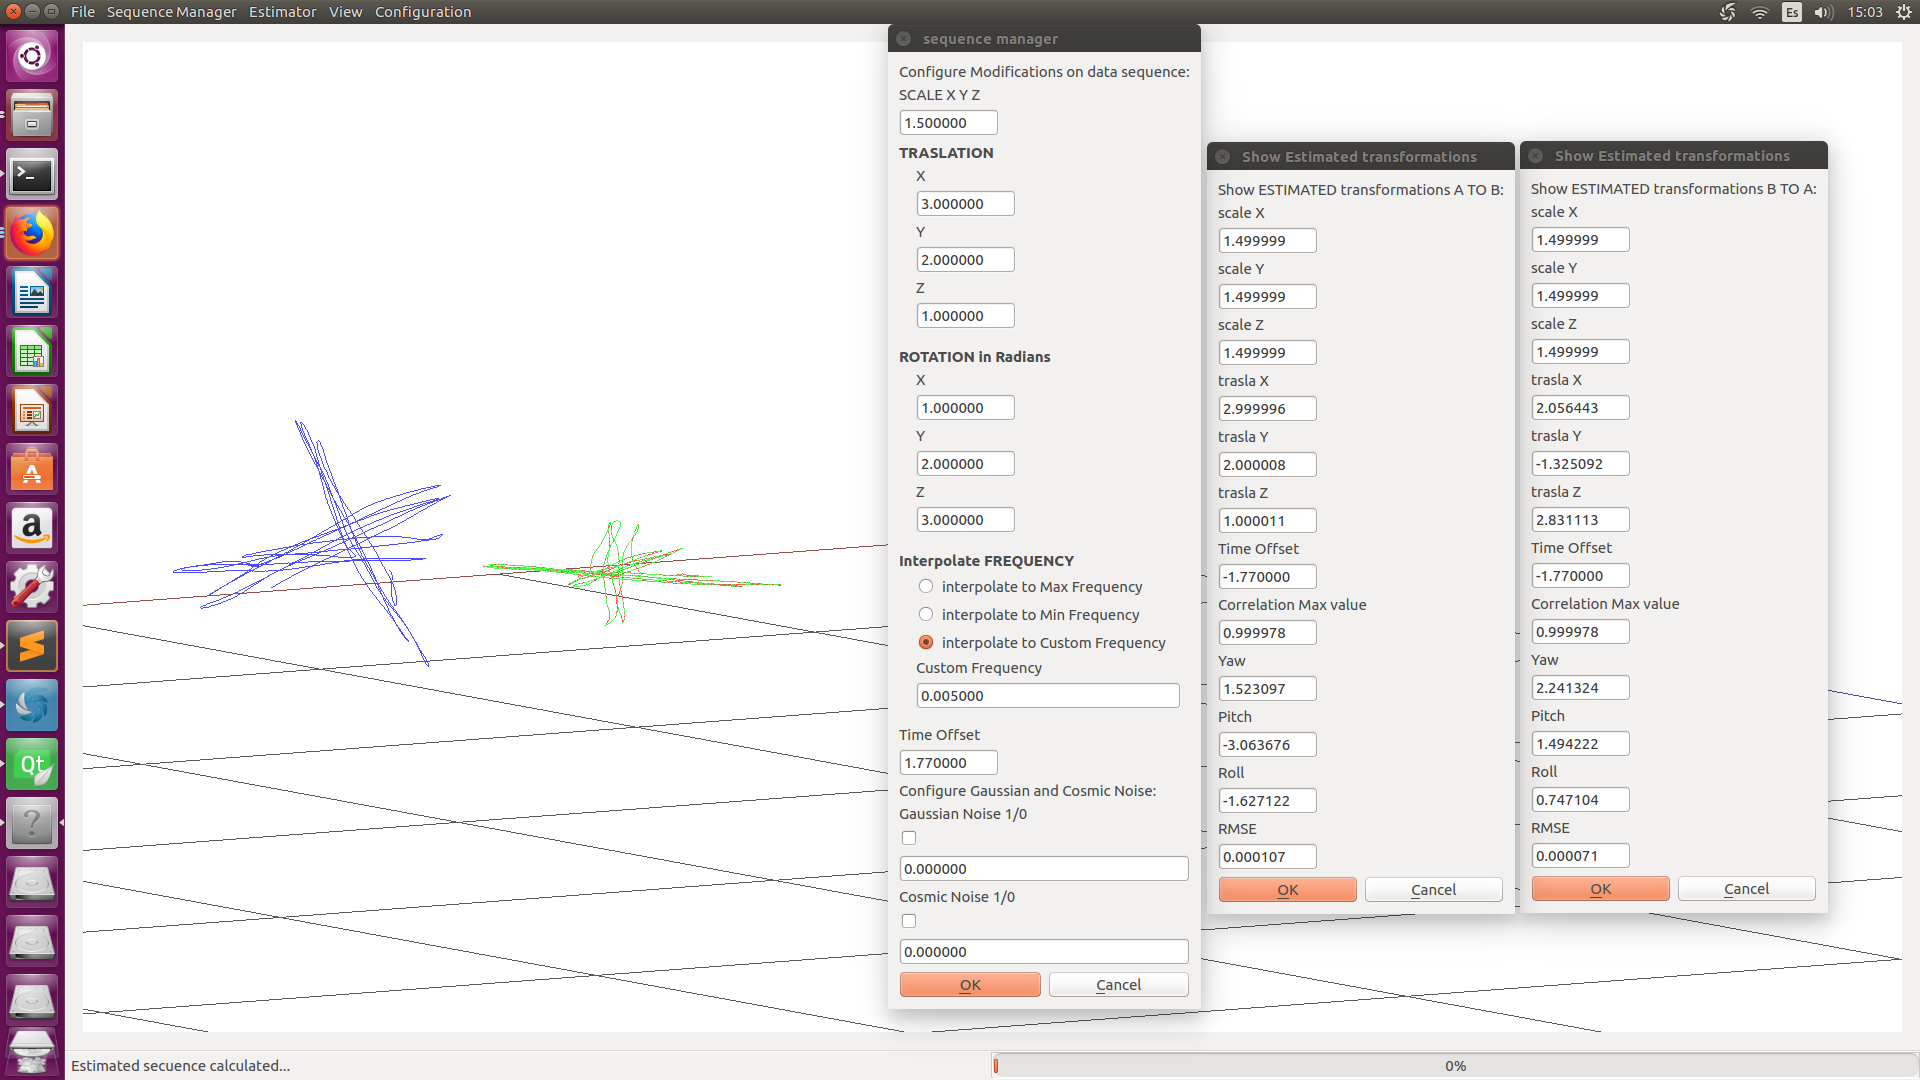
\includegraphics[height=8.0cm,width=12.0cm]{img/cap6/ScaleTraslaRotaFrecTimeOffset.png}}
\hspace{0.5cm}

\end{center}

\caption{Gráfico que muestra los resultados de la estimación de un cambio de escala, traslación, rotación, frecuencia y offset.}
\end{figure}


\begin{figure}[H]
\begin{center}
\subfigure[]{\label{fig:opciones de View}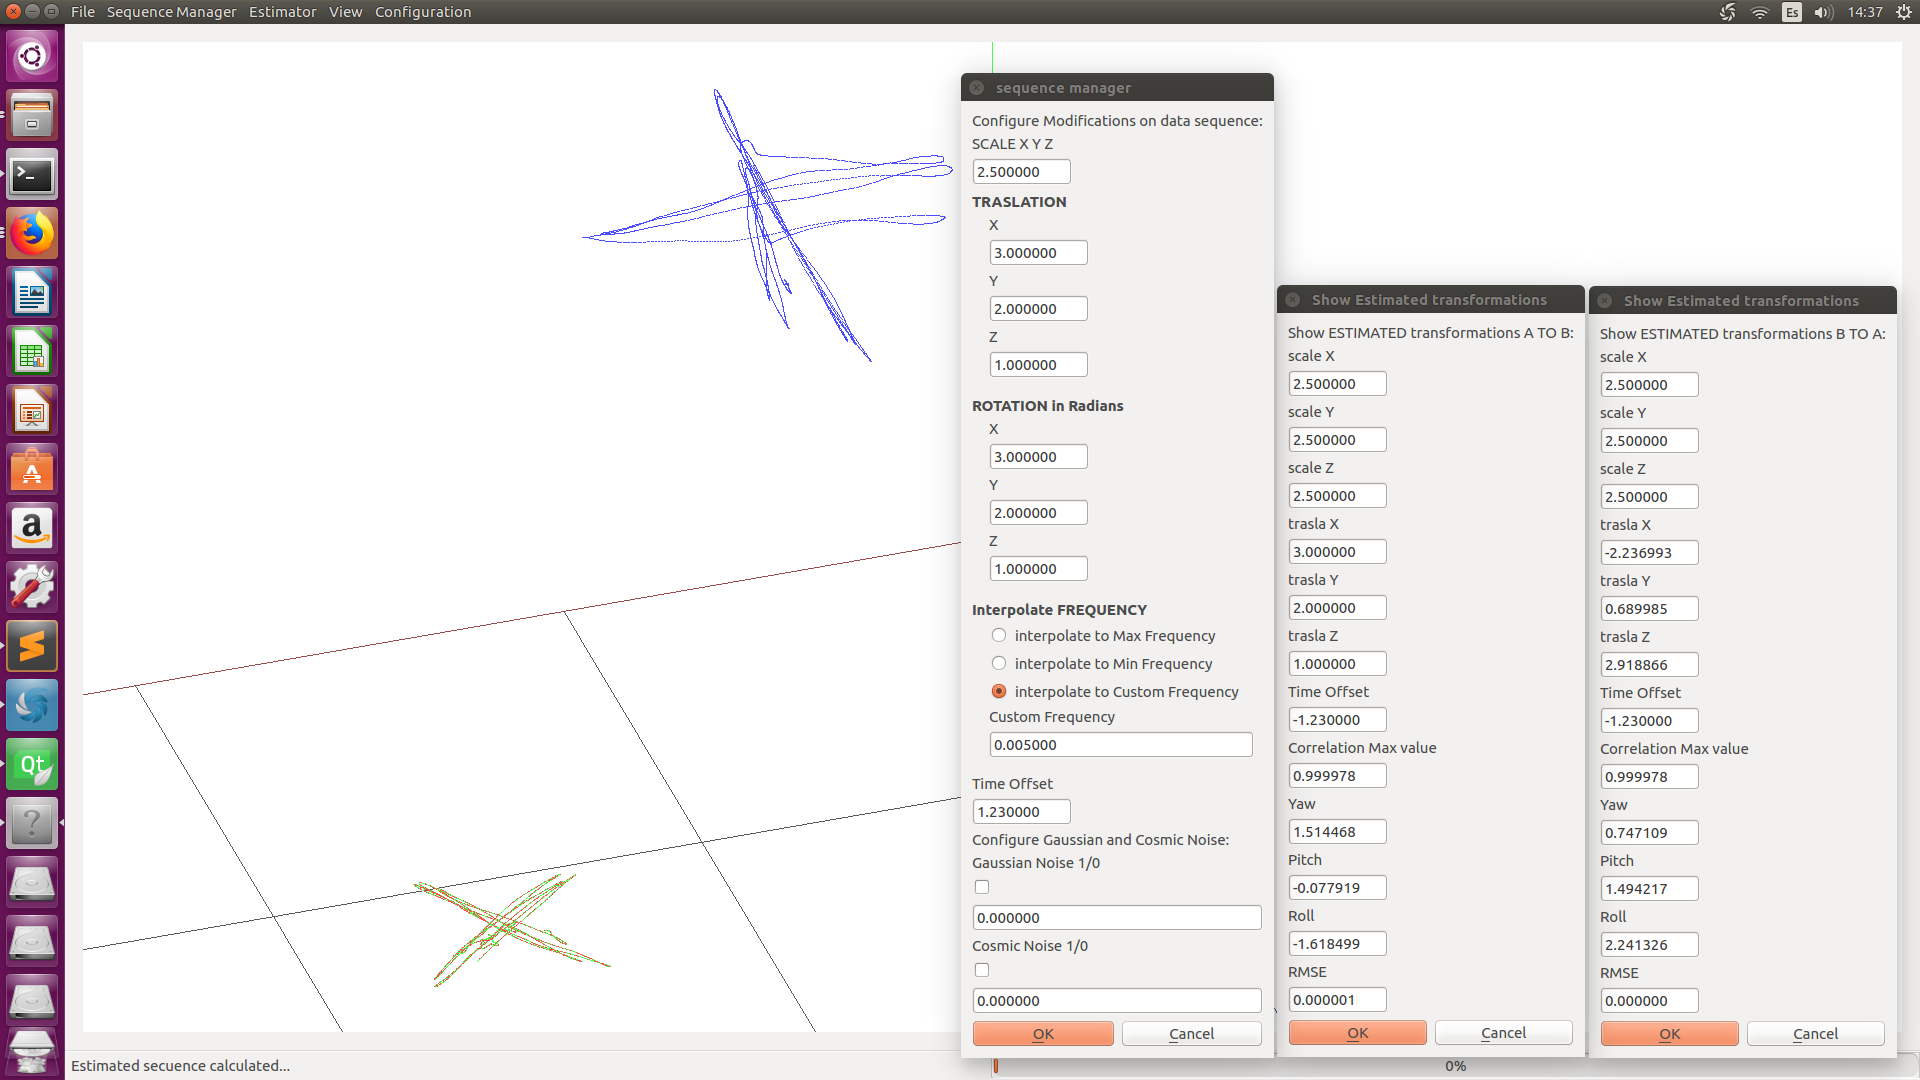
\includegraphics[height=8.0cm,width=12.0cm]{img/cap6/ScaleTraslaRotaFrecTimeOffset2.png}}
\hspace{0.5cm}

\end{center}

\caption{Gráfico que muestra los resultados de la estimación de un cambio de escala, traslación, rotación, frecuencia y offset.}
\end{figure}



\begin{figure}[H]
\begin{center}
\subfigure[]{\label{fig:opciones de View}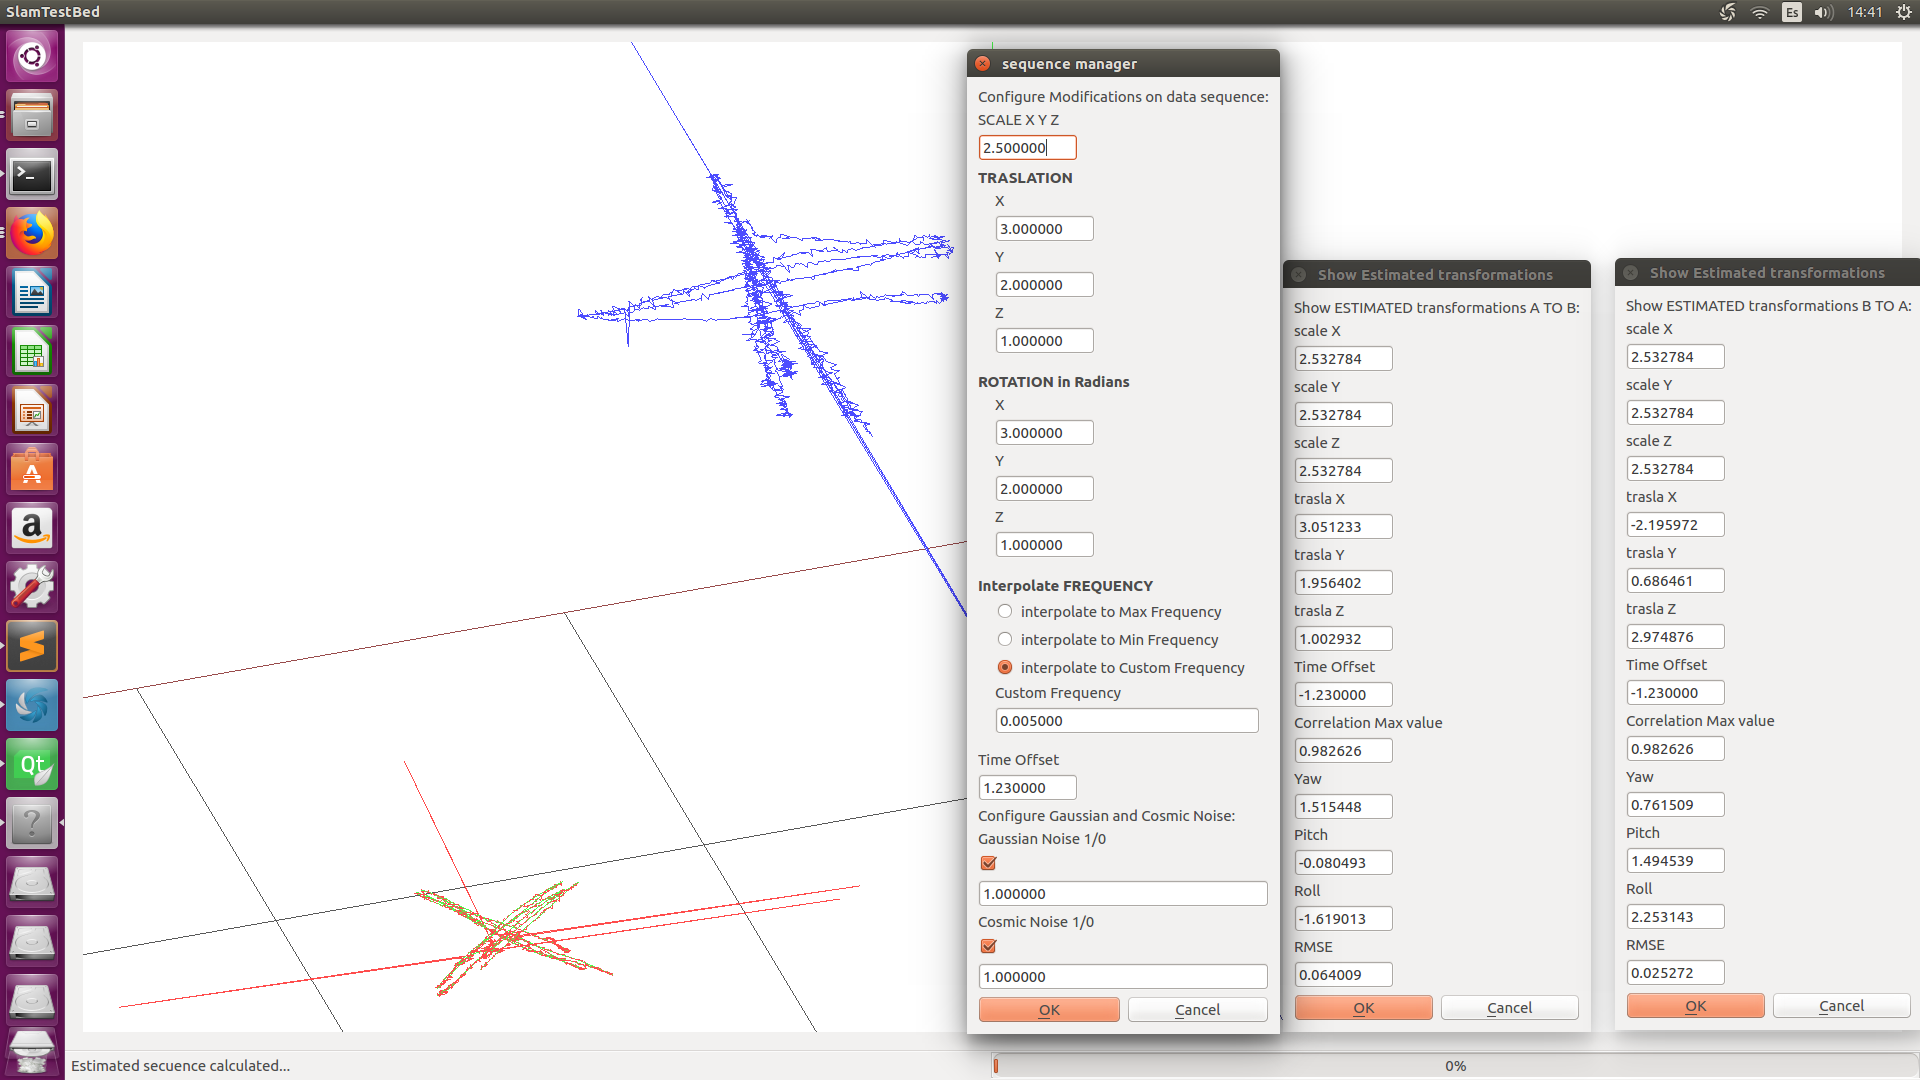
\includegraphics[height=8.0cm,width=12.0cm]{img/cap6/ScaleTraslaRotaFrecTimeOffsetGNoiseCNoise.png}}
\hspace{0.5cm}

\end{center}

\caption{Gráfico que muestra los resultados de la estimación de un cambio de escala, traslación, rotación, frecuencia, Offset, Ruido Gausiano y Ruido Cósmico.}
\end{figure}




\begin{figure}[H]
\begin{center}
\subfigure[]{\label{fig:opciones de View}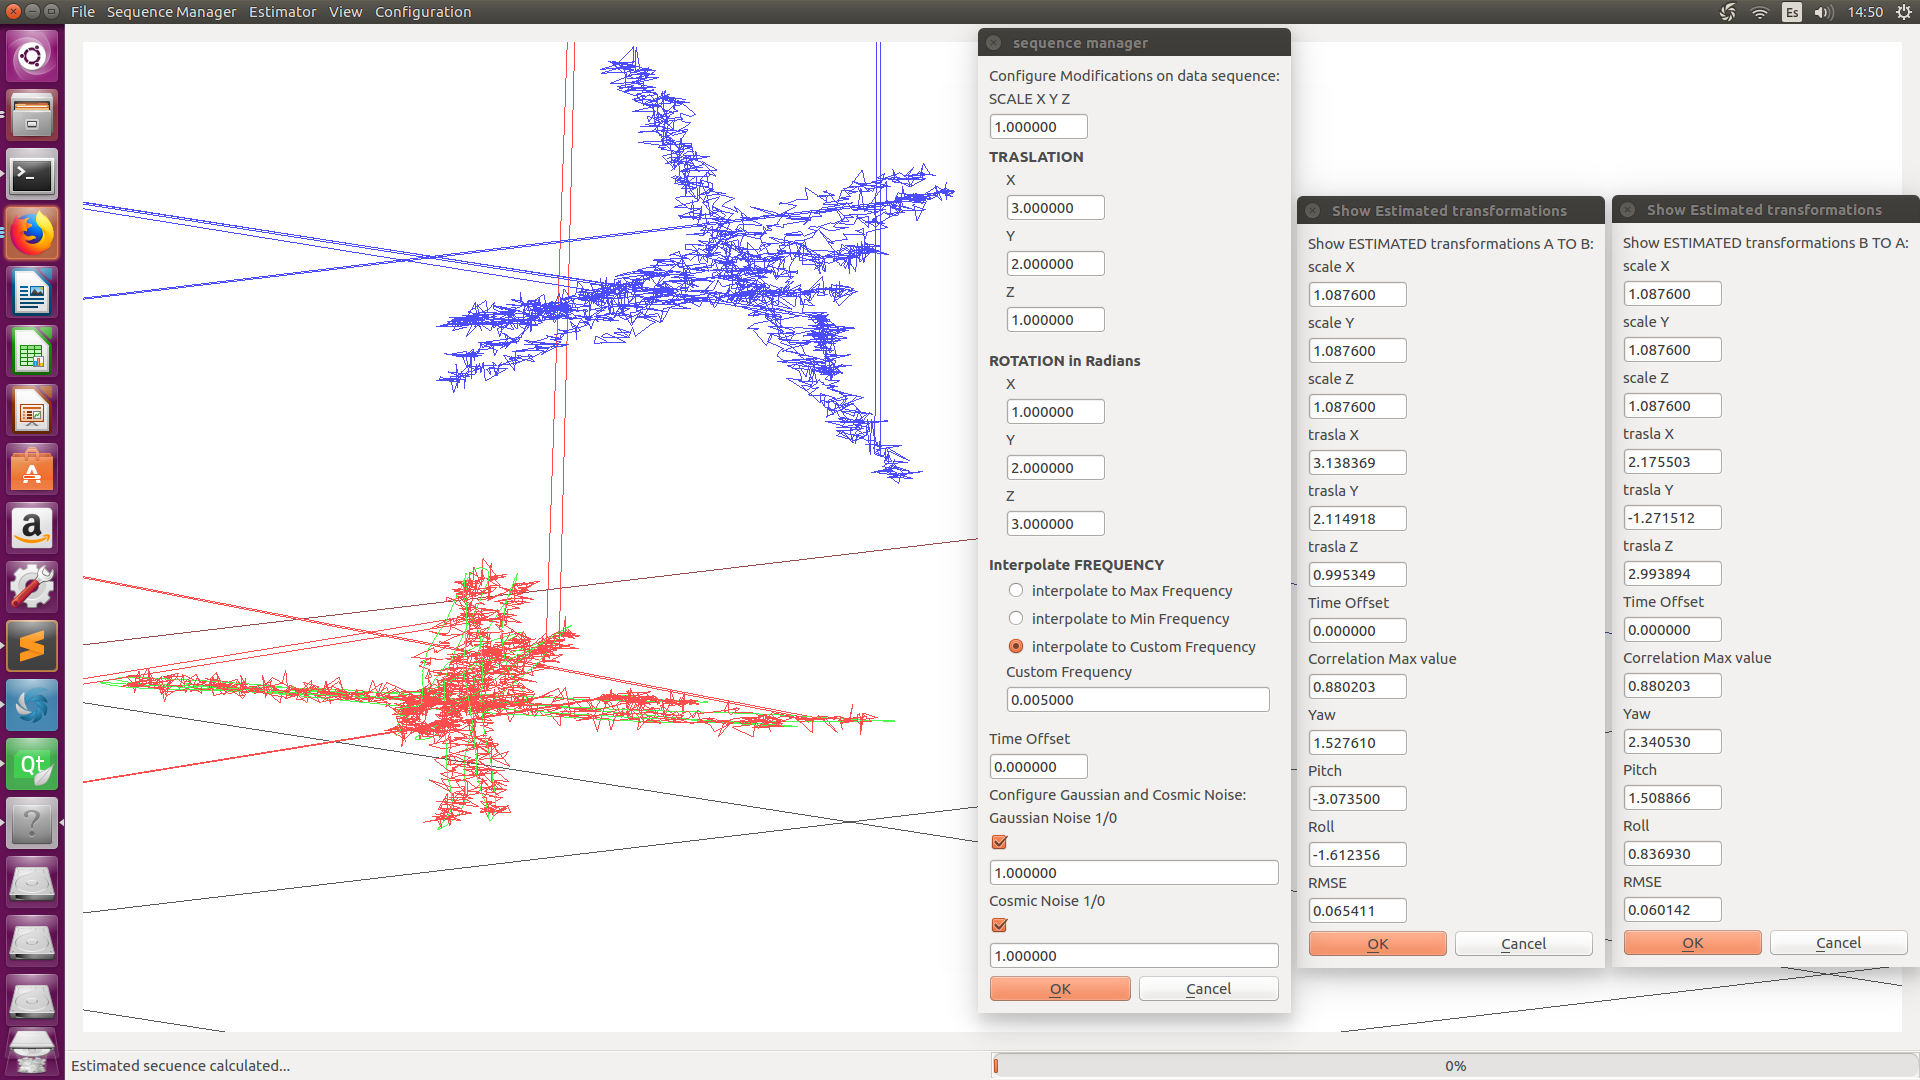
\includegraphics[height=8.0cm,width=12.0cm]{img/cap6/TraslaRotaFrecGnoiseCnoise.png}}
\hspace{0.5cm}

\end{center}

\caption{Gráfico que muestra los resultados de la estimación de un cambio de traslación, rotación, frecuencia, Ruido Gaussiano y Ruido Cósmico.}
\end{figure}


Por último también mostraremos como SLAMTestBed es capaz de operar con 2 datasets diferentes , es decir en este caso , el seguno dataset no será el resultado de aplicar el módulo de transformación sobre el primer dataset.

\begin{figure}[H]
\begin{center}
\subfigure[]{\label{fig:opciones de View}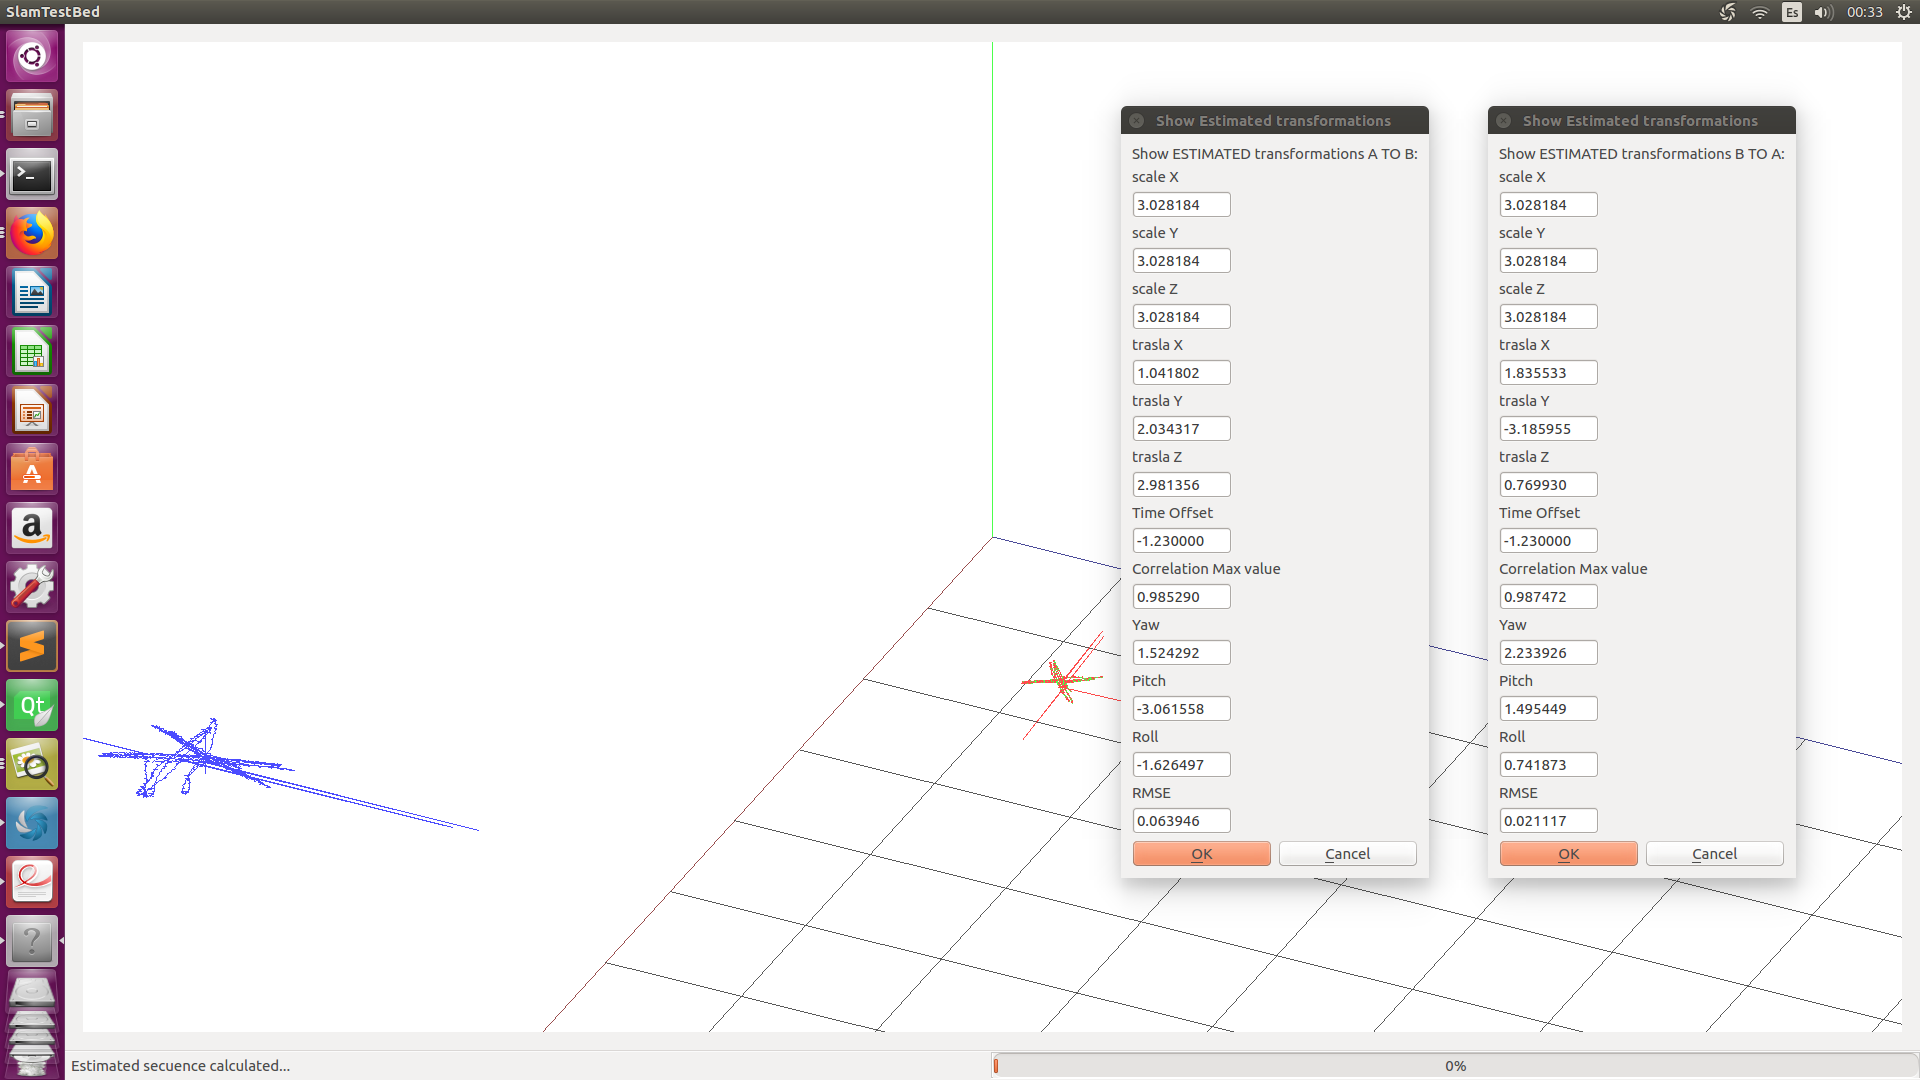
\includegraphics[height=8.0cm,width=12.0cm]{img/cap6/LoadTwoDataSets.png}}
\hspace{0.5cm}

\end{center}

\caption{Gráfico que muestra los resultados de la estimación de la transformación del datasetA en el datasetB y viceversa.}
\end{figure}


\begin{figure}[H]
\begin{center}
\subfigure[]{\label{fig:opciones de View}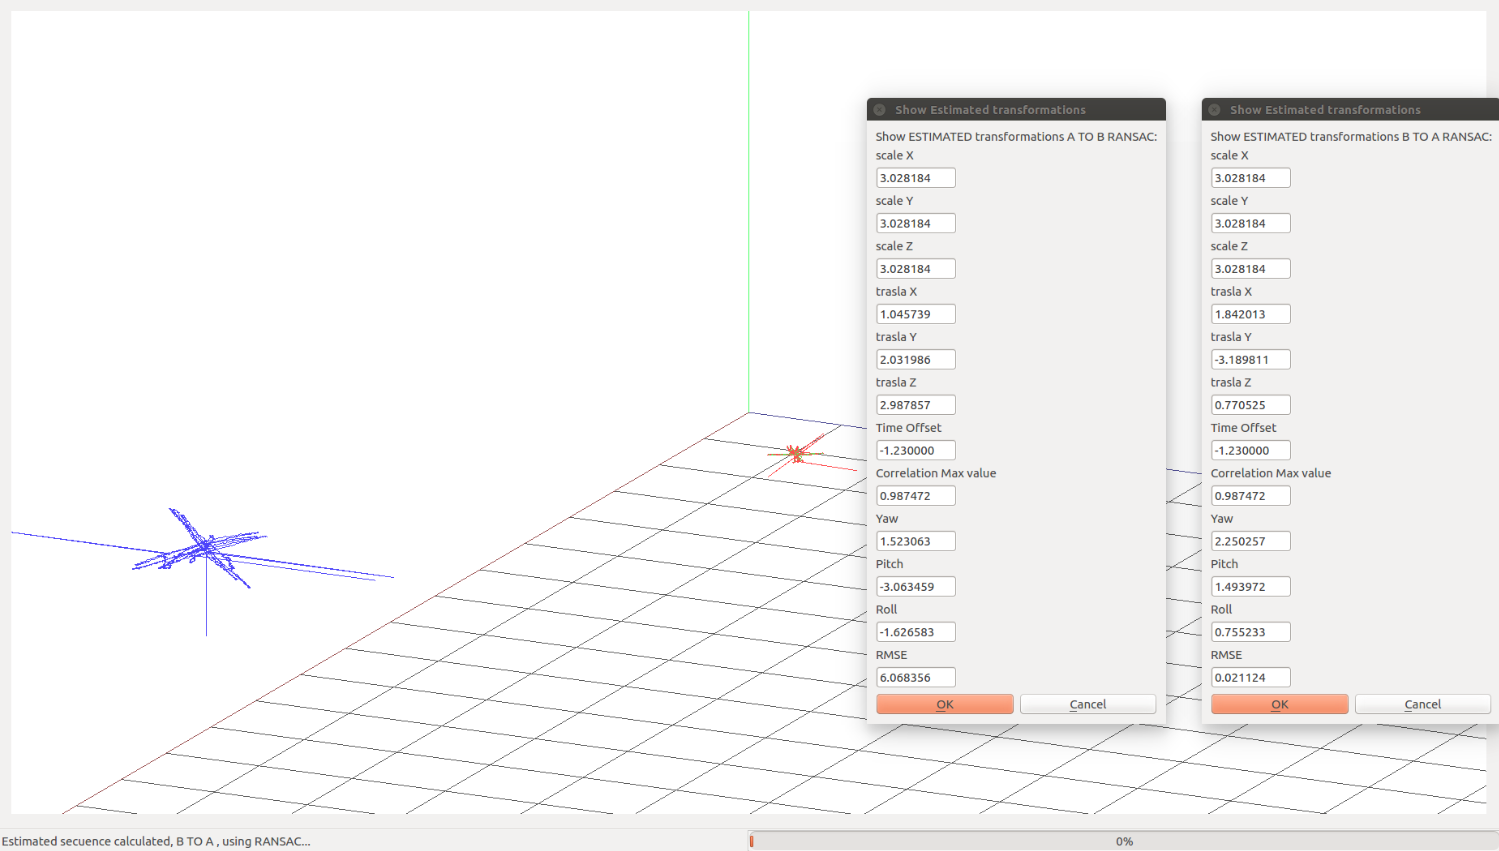
\includegraphics[height=8.0cm,width=12.0cm]{img/cap6/LoadTwoDataSets_RANSAC.png}}
\hspace{0.5cm}

\end{center}

\caption{Gráfico que muestra los resultados de la estimación de la transformación del datasetA en el datasetB y viceversa, utilizando RANSAC.}
\end{figure}




